I dette afsnit vil vi først og fremmest undersøge nogle vigtige egenskaber ved $\mathbb{R}$, der er nødvendige for en stringent opbygning af integrationsteorien.
Derefter indfører vi grundlæggende teori om topologi for $\mathbb{R}$, som vi senere skal bruge til at definere kontinuitet samt grænseværdien for en funktion.\footnote{Afsnittet er baseret på \cite{Rudin1976}, s. 3-33. Vi nøjes dog med at kigge på delmængder af $\mathbb{R}$, hvor Rudins bog behandler teorien mere generelt via metriske rum.}

\subsection{Supremum-egenskaben}%
  \label{sub:Supremum-egenskaben}

\begin{definition}[label=def:overtal]{Overtal, undertal}{}
  Antag, at $A \subseteq \mathbb{R}$. 
  Hvis der eksisterer $y \in \mathbb{R}$ sådan at $x \leq y$ for alle $x \in A$, så siges $A$ at være opad begrænset, og $y$ kaldes et overtal for $A$. 

  Hvis der eksisterer $z \in \mathbb{R}$ sådan at $x \geq z$ for alle $x \in A$, så siges $A$ at være nedad begrænset, og $z$ kaldes et undertal for $A$. 
\end{definition}

Imidlertid, kan det også være interessant at kunne sige noget om, hvorvidt et bestemt overtal er det mindste overtal og et bestemt undertal er det største undertal.

\begin{definition}[label=def:sup]{Supremum, infimum}{}
  Antag, at $A \subseteq \mathbb{R}$. Et element $y \in \mathbb{R}$ kaldes supremum eller mindste overtal af $A$ og betegnes $\sup A$, hvis $y$ har følgende egenskaber:
  \begin{itemize}
    \item $y$ er et overtal for $A$.
    \item $y \leq z$ for alle overtal $z$ af $A$. 
  \end{itemize}
  Et element $\beta \in \mathbb{R}$ kaldes infimum eller største undertal af $A$ og betegnes $\inf A$, hvis $\beta$ har følgende egenskaber:
  \begin{itemize}
    \item $\beta$ er et undertal for $A$.
    \item $\beta \geq \alpha$ for alle undertal $\alpha$ af $A$. 
  \end{itemize}
\end{definition}

\begin{example}[label=exa:supinf]{Supremum og infimum af mængder}{}
  Betragt mængderne
  \[
  A=\{ a \in \mathbb{R}:a \leq 1 \}\quad \text{og} \quad B=\{ b \in \mathbb{R}: b>0 \}. 
  \] 
  Vi har så $\sup A=1$ og $\inf B=0$.
  Derudover er mængden $A$ ikke nedad begrænset og mængden $B$ er ikke opad begrænset. 
\end{example}

Bemærk, at $\sup A \in A$, hvor $\inf B \not\in B$.
Det næste eksempel viser, at en ikke-tom opad begrænset delmængde af $\mathbb{Q}$ kan have supremum, der ikke er i $\mathbb{Q}$. 

\begin{example}[label=exa:supQ]{Ikke-tom opad begrænset delmængde af $\mathbb{Q}$ uden supremum i $\mathbb{Q}$}{}
  
\end{example}

Eksempel \ref{exa:supQ} motiverer den næste sætning, som vi her ikke vil bevise, da beviset er relativt langt og ikke interessant for vores foretagende.
Sætningen er dog en følge af måden, hvorpå $\mathbb{R}$ er konstrueret.\footnote{$\mathbb{R}$ kan konstrueres fra $\mathbb{Q}$ via Dedekind-snit. \cite{Rudin1976}, s. 17-21}

\begin{theorem}{$\mathbb{R}$ har supremum-egenskaben}{}
  Antag, at $A \in \mathbb{R}$, $A \neq \emptyset$ og $A$ er opad begrænset. 
  Så eksisterer $\sup A \in \mathbb{R}$.
\end{theorem}

Denne egenskab ved $\mathbb{R}$ kaldes for supremum-egenskaben. 
Bemærk, at en alternativ tilgang her kunne være at definere $\mathbb{R}$ ud fra supremum-egenskaben og derefter bevise $\mathbb{R}$'s eksistens ved konstruktion.
Vi vil nu ud fra supremum-egenskaben af $\mathbb{R}$ vise, at $\mathbb{R}$ også må have infimum-egenskaben. 

\begin{theorem}[label=theo:]{$\mathbb{R}$ har infimum-egenskaben  }{}
  Antag, at $A \in \mathbb{R}$, $A \neq \emptyset$ og $A$ er nedad begrænset.
  Så eksisterer $\inf A \in \mathbb{R}$.
\end{theorem}
\begin{proof} 
  Lad 
  \[
  B=\{ b \in \mathbb{R} : b \leq a \text{ for alle } a \in A \}.
  \]  
  Så er $B$ mængden af alle undertal for $A$.
  Siden $A$ er nedad begrænset, så er $B$ ikke tom.
  Siden $A \neq \emptyset$, så er $B$ opad begrænset. 
  Fra supremum-egenskaben eksisterer da $\sup B \in \mathbb{R}$. 

  Per definition \ref{def:sup} har vi så, at $\sup B \leq a$ for alle $a \in A$ (fordi alle elementer af $A$ er overtal for $B$). 
  Siden $\sup B$ også er større end eller lig alle undertal for $A$, så må $\sup B=\inf A$. 
\end{proof}

\subsection{Topologi i $\mathbb{R}$}%
  \label{sub:Topologi i R}
Det skal bemærkes, at når vi arbejder med $\mathbb{R}$, så kan ordene \textit{punkt} og \textit{tal} bruges i flæng.
Begge ord referer i dette tilfælde til elementerne i $\mathbb{R}$.
  
\begin{definition}[label=def:omegn]{Omegn}{}
  Antag $p \in \mathbb{R}$. 
  Så er en omegn af et punt $p$ en mængde 
  \[
  N_r(p)=\{ q \in \mathbb{R}:\abs{q-p} < r \}, \quad \text{ hvor }r \in \mathbb{R}^+. 
  \] 
  Tallet $r$ kaldes for radius af omegnen $N_r(p)$. 
\end{definition}
Med andre ord, er en omegn af et punkt $p$ mængden af alle punkter indenfor en given afstand fra $p$.
Dette ses illustreret i \cref{fig:omegn}.
\begin{figure}[H]
\begin{center}
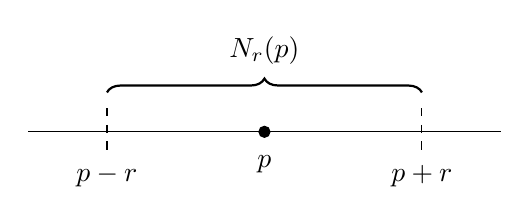
\begin{tikzpicture}
  \centering
    %\tikzstyle{point}=[circle,thick,draw=black,fill=black,inner sep=0pt,minimum width=4pt,minimum height=4pt]
    %\node [point] at (0,0) {};
    \filldraw[black] (0,0) circle (2pt) node[below=5pt]{$p$};
    \draw (-3,0) -- (3,0);
    \draw [dashed] (-2,0.3) -- (-2,-0.3) node[anchor=north]{$p-r$};
    \draw [dashed] (2,0.3) -- (2,-0.3) node[anchor=north]{$p+r$};
    \draw [decorate, decoration = {brace,amplitude=5pt}, thick] (-2,0.5) -- (2,0.5) node[midway,yshift=3.5ex]{$N_r(p)$};
    %\draw [decorate,decoration={brace,amplitude=5pt,mirror,raise=4ex}] (1,0) -- (5,0) node[midway,yshift=-3em]{Konvergenzbereich};
\end{tikzpicture}
\end{center}
  \caption{Illustration af en omegn $N_r(p)$}
\label{fig:omegn}
\end{figure}

\begin{definition}[label=def:fortætningspunkt]{Fortætningspunkt}{}
  Antag, at $A \subseteq \mathbb{R}$.
  Et punkt $p \in \mathbb{R}$ er et fortætningspunkt af mængden $A$, hvis der for alle omegne $N_r(p)$ eksisterer et punkt $q \neq p$ i omegnen sådan at $q \in A$. 
\end{definition}




